%-------------------------------------------------------------------------------
% LATEX TEMPLATE ARTIKEL
%-------------------------------------------------------------------------------
% Dit template is voor gebruik door studenten van de de bacheloropleiding 
% Informatica van de Universiteit van Amsterdam.
% Voor informatie over schrijfvaardigheden, zie 
%                               https://practicumav.nl/schrijven/index.html
%
%-------------------------------------------------------------------------------
%	PACKAGES EN DOCUMENT CONFIGURATIE
%-------------------------------------------------------------------------------

\documentclass{uva-inf-article}
\usepackage[dutch]{babel}

\usepackage[style=authoryear-comp]{biblatex}
\addbibresource{references.bib}

\usepackage{pdfpages}

%-------------------------------------------------------------------------------
%	GEGEVENS VOOR IN DE TITEL, HEADER EN FOOTER
%-------------------------------------------------------------------------------

% Geef je artikel een logische titel die de inhoud dekt.
\title{The quest to finding the best SNNI}

% Vul de naam van de opdracht in zoals gegeven door de docent en het type 
% opdracht, bijvoorbeeld 'technisch rapport' of 'essay'.
\assignment{Projectplan}
\assignmenttype{}

% Vul de volledige namen van alle auteurs in en de corresponderende UvAnetID's.
\authors{Jorit Prins}
\uvanetids{12862789}

% Vul de naam van je tutor, begeleider (mentor), of docent / vakcoördinator in.
% Vermeld in ieder geval de naam van diegene die het artikel nakijkt!
\supervisors{Zoltan Mann}
% \mentor{Marco Brohet}
\docent{}

% Vul hier de naam van je tutorgroep, werkgroep, of practicumgroep in.
\group{}

% Vul de naam van de cursus in en de cursuscode, te vinden op o.a. DataNose.
\course{Afstudeerproject}
\courseid{}

% Dit is de datum die op het document komt te staan. Standaard is dat vandaag.
\date{\today}

%-------------------------------------------------------------------------------
%	VOORPAGINA 
%-------------------------------------------------------------------------------

\begin{document}
\maketitle

%-------------------------------------------------------------------------------
%	INHOUDSOPGAVE EN ABSTRACT
%-------------------------------------------------------------------------------
% Niet toevoegen bij een kort artikel, zeg minder dan 10 pagina's!

%TC:ignore
%\tableofcontents
%\begin{abstract}
%\end{abstract}
%TC:endignore

%-------------------------------------------------------------------------------
%	INHOUD
%-------------------------------------------------------------------------------
% Hanteer bij benadering IMRAD: Introduction, Method, Results, Discussion.

%[hebben veelbelovende resultaten en staan aan de voorgrond/voorsprong van] 
\section{Relevance}
The recent rise in Big Data increased the data exchange on the internet. With more and more computer resources available, researchers quickly started to utilise the possibilities of machine learning (ML) to analyse the data.  Techniques like neural networks (NN) are promising ways to scientific breaktroughs. Machine learning has a wide varity of applications for classification such as traffic analysis, image recognition, intrusion detection,  spam detection, medical or genomics predictions,  financial predictions and face recognition \parencite{Dowlin2017, Islam2011, Bachrach16, Kaiming215}

The use of ML typically consists of two phases: training and inference. In the first phase a NN is trained by feeding an extensive dataset to find the best parameters. NNs used for machine learning have to be maintained, evaluated and the training phase is often a tedious and time exhausting process. In the inference phase an input is applied to the trained NN. Because of the time consuming process of creating a NN, machine learning as a service (MLaaS) became popular. In MLaaS, a company offers a pre-trained NN to the clients. Now, clients only need to worry about the inference phase.

However, MLaaS offers great threats to privacy. To train the model as accurately as possible a NN needs access to a large amount of precise data from clients, which may consist of sensitive information. Thus, clients may be reluctant to provide the NNs with their data. Other features, irrelevant to the prediction task, could also be derived from this data \parencite{Nasr2019}. On the inference phase, input from the client to the NN can also be confidential. On the other hand, owners of a NN could be worried that an adversary could steal (parameters of) their (often costly) NN. Furthermore, the result of the NN could also be confidential resulting in the need to retain this information from unauthorized parties. 

A typical MLaaS situation consist of two parties: the client holding an input \textit{x} and a company holding neural network \textit{f}. For this research we will focus on the inferrence part. The client wants to know the applied input \textit{f(x)} while keeping the sensitive contents of \textit{x} and the result \textit{f(x)} private from the company. The company wants to hold the intelectual property \textit{f} private while still giving the opportunity to the client to use \textit{f}. The secure neural network inference (SNNI) problem entails calculating the applied input \textit{f(x)} while still holding all the above security requirements. 

No general implementation of an SNNI has been widely accepted to the authors knowledge. Rapid progress in this area has made it hard to get a good overview of technological advances. Mann et al. \yearcite{Mann22} has summarized several proposed approaches for SNNI. However, these approaches are often proof-of-concept and are not thoroughly tested. Moreover, the performance is often only tested on basic measures like efficiency or privacy and tests are on a basic setup (laptop to local server).

Metrics like power usage are important in the internet of things (IoT), where clients are constrained to use devices with limited performance. This limits the applicability of certain approaches that put burden on the client, and the server side should be able to handle many requests.  

\section{Research question(s) and Method}
To contribute to the prior research in this area, this paper will focus on testing one (or more) already existing open source implementations, for example ABY2.0 \parencite{ABY20}, Chameleon \parencite{Chameleon}, Cheetah \parencite{Cheetah}, CrypTFlow2 \parencite{CrypTFlow2} and Delphi \parencite{Delphi} on their power usage. 

To select an existing approach we need to set our constraints: the approach should be available for everyone and there should already be an existing implementation that is open source. To select the approach to test further research lies is in the following research question:
\begin{quote}\emph{RQ1: what is needed to make a SNNI approach good and realistic (e.g. setup and computing power)?}\end{quote}
\textit{RQ1} will be answered with an extensive literature research. After this literature research we can also answer the following question:
\begin{quote}\emp{RQ2: what are sufficient metrics to test a SNNI approach (e.g. power usage)?}\end{quote} and
\begin{quote}\emp{RQ3: how can we test these metrics on our SNNI}\end{quote}
We can start selecting our desired implementation once we have answerd \textit{RQ1}. As soon as we have selected our SNNI approach, we can start downloading the SNNI and making it work at our own setup. Once we have got it all working we can start testing the implementation. We test the implementation with the answers found on research question \textit{RQ2}. A small literature search can be done on what databases to use for our testing puroposes, resulting in the following question:
\begin{quote}\emp{RQ3: what databases should we use for our testing?}\end{quote}

\section{Schedule} 
(will come once research questions are formulated good enough => see email)
% 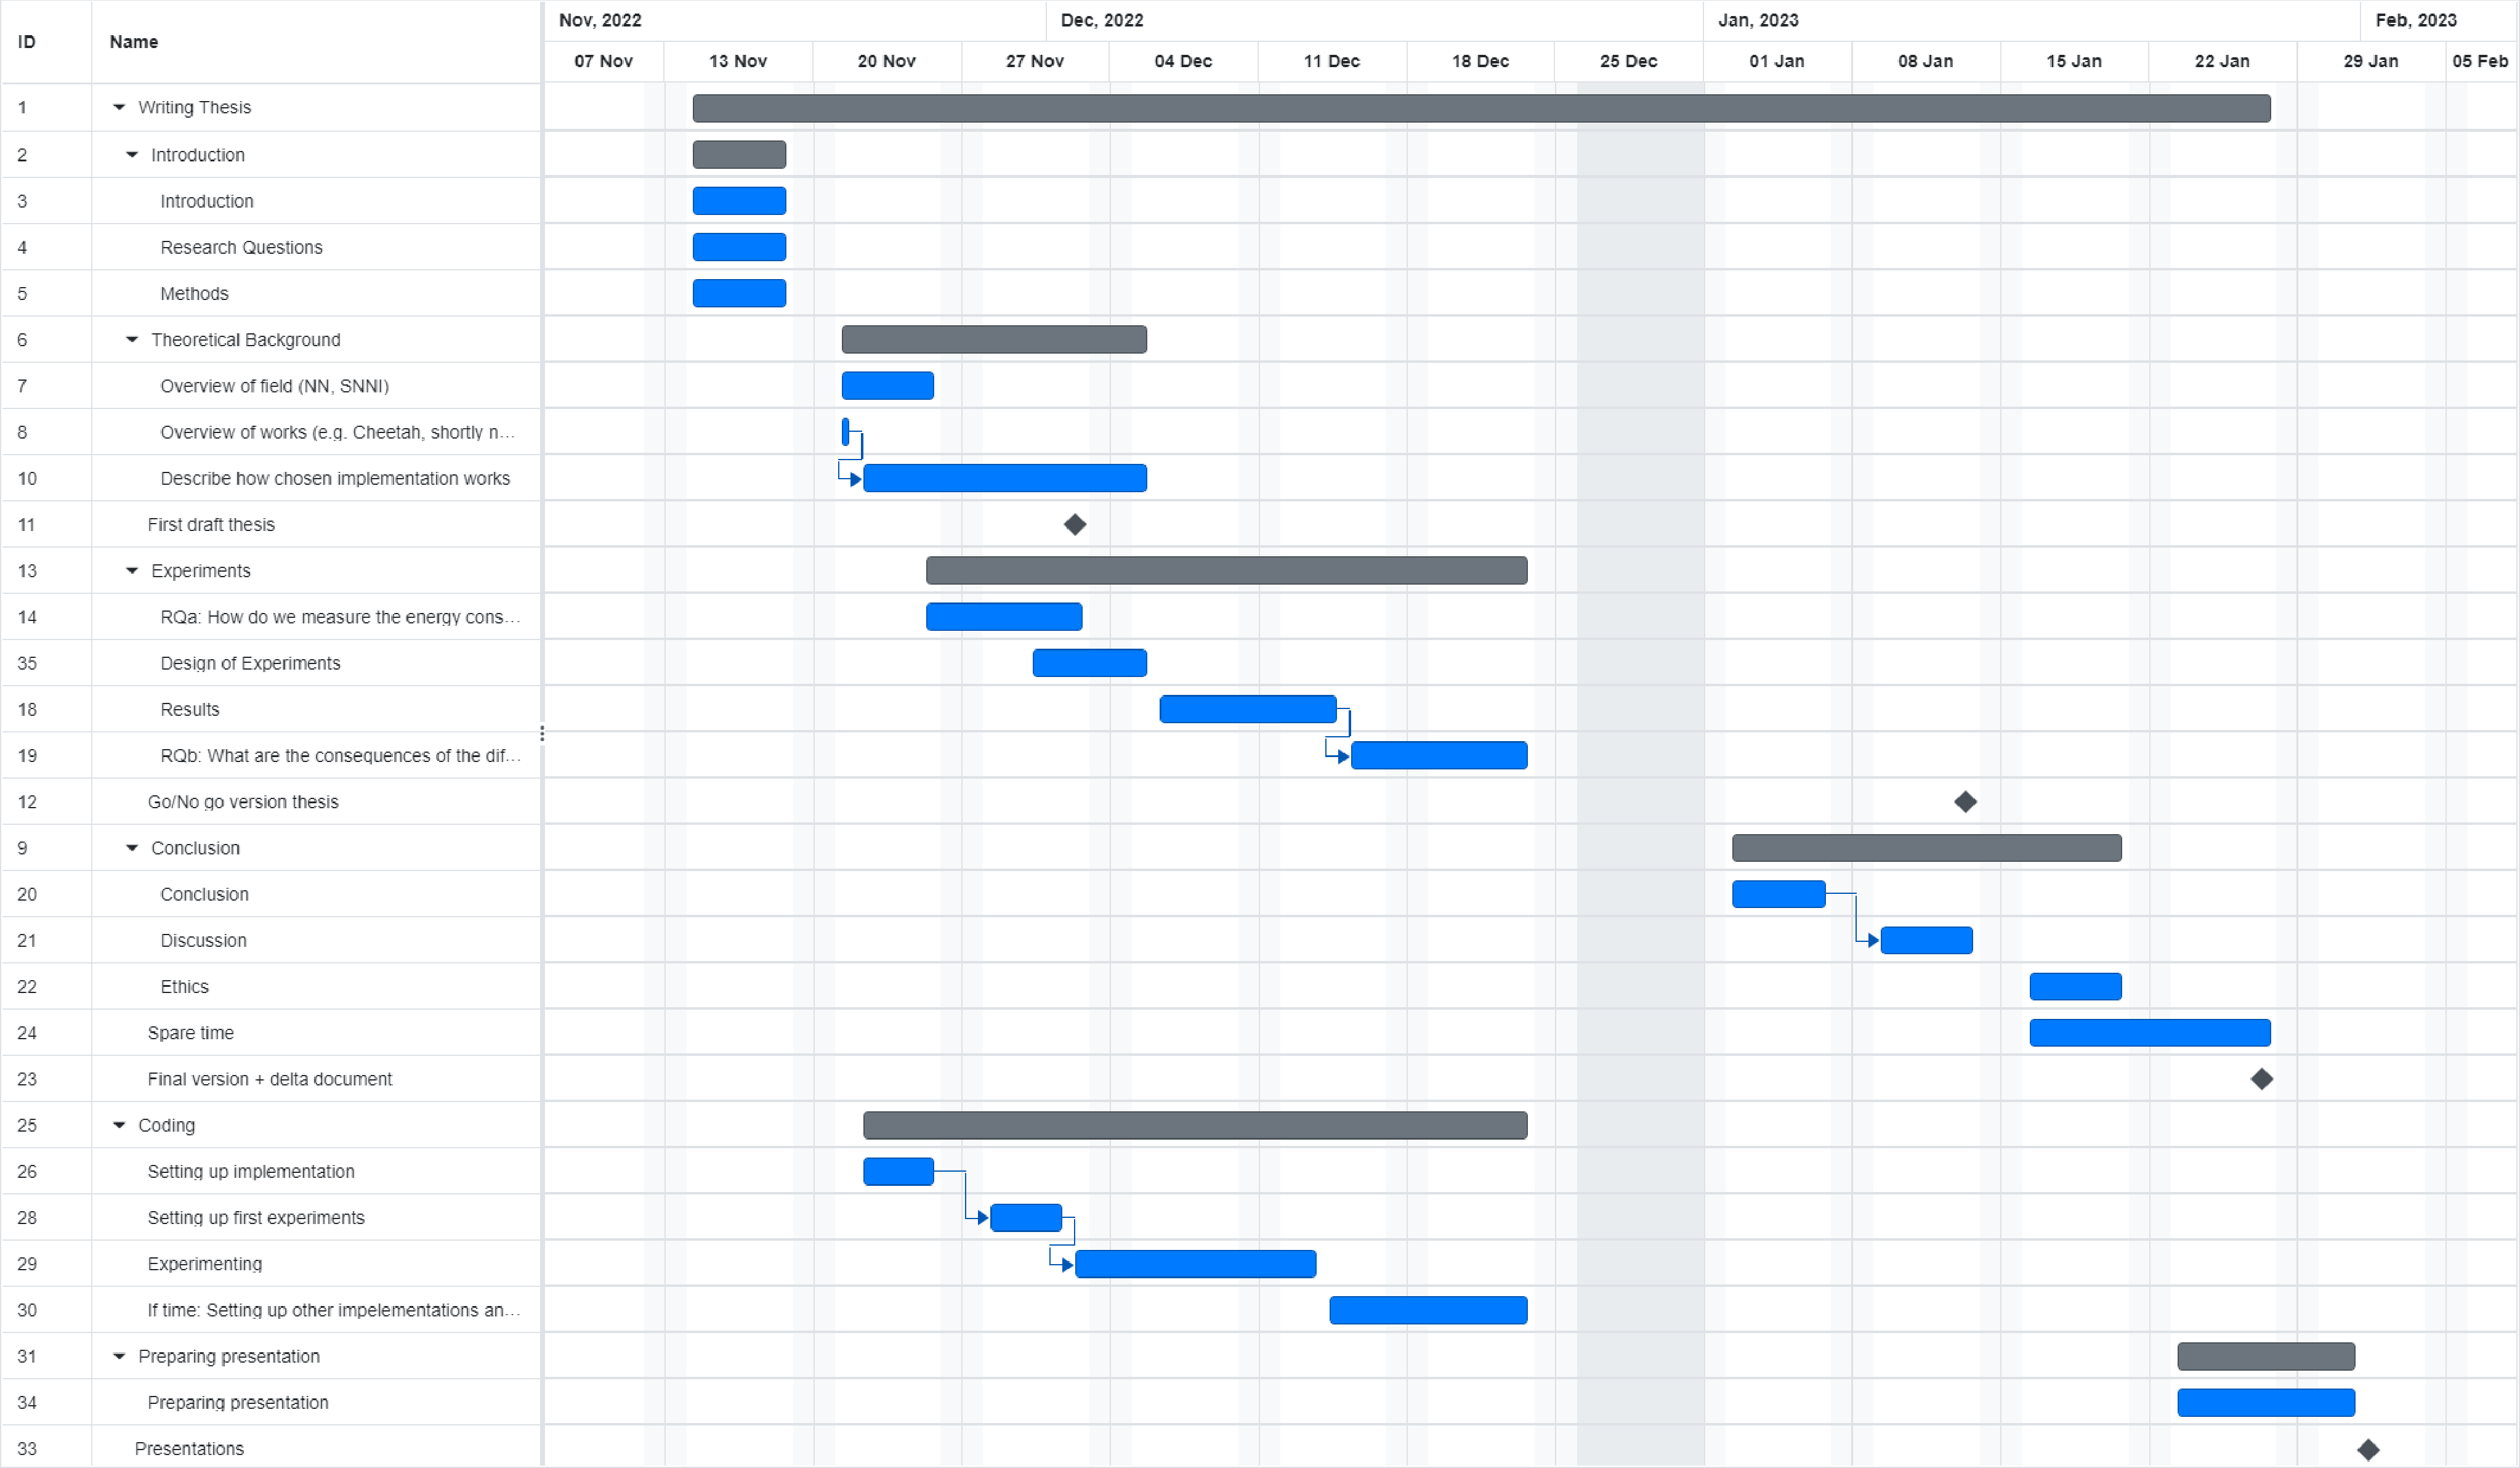
\includepdf[pages=-,angle=270]{Gantchart_Thesis.pdf}


% \subsectionauthor[Voornaam Achternaam]{Paragraaf met auteur}
% \lipsum[2-3]

%-------------------------------------------------------------------------------
%	REFERENTIES
%-------------------------------------------------------------------------------
\newpage
\printbibliography

%-------------------------------------------------------------------------------
\end{document}